\chapter{Text detection}
\label{ch:detection}

The challenges presented in \autoref{sec:challenges} make it clear that a classical approach is unsuitable for our problem. As such, we direct our attention towards the modern, robust architectures of Convolutional Neural Networks (CNN) \citep{leCun_CNN}. In particular, we take inspiration from the great advances in object detection and we will treat text like a regular object which can be found anywhere in the image.

\Autoref{sec:faster_rcnn} introduces the first architecture we tested, the \FRCNN{} \citep{faster_rcnn}, as a mean of establishing a baseline. Then we explain how we produce data for training the architecture in \autoref{sec:detection_data} and how intermediate results drive us to more advanced data generation techniques. Then, \autoref{sec:ctpn} presents a more powerful architecure for text detection, the \emph{Connectionist Text Proposal Network}(\CTPN{}, \citet{ctpn}). \todo{Specify about detection results. First, we need to define what kind of results to present. Maybe just very short FRCNN vs CTPN on final constats => need to define benchmark.}


%========================================================================================

\section{Faster R-CNN}\label{sec:faster_rcnn}

	The task of object detection builds upon that of image classification. Architectures based on region proposals (see \autoref{sec:related_detection}) can be seen as a two stage algorithm: the first part extracts possible object bounding boxes as a sub-image of the input, while the second one predicts the class associated with each candidate. It is of no surprise then that object detection greatly benefits from the super-human accuracy of deep neural networks \citep{superhuman_classif}. We chose to pair the \FRCNN{} detection architecture with the \RESNET{} feature extractor \citep{resnet}, since this has been proven as a good trade-off between detection accuracy and speed on the standard challenge of ILSCVR \citep{detection_benchmark}. In what follows we present the main building blocks of this architecture.

	%----------------------------------------------------------------------------------------

	\subsection{Feature extraction}\label{sec:resnet}
		In order to perform detection on an input image, we first need to extract representative high-level features from the raw pixel values. To this end, we employ the \RESNET{} convolutional architecture which has won many competitions in classification, detection and segmentation.

		The novelty of this approach\footnote{\todo{Should I dedicate a subsection to describe how (Conv) Neural Nets work?}} relies in forcing the network to learn a \emph{residual} mapping \(\mathcal{F}(\ve{x}) := \mathcal{H}(\ve{x}) - \ve{x}\), where \(\mathcal{H}(\ve{x})\) represents a desired mapping from input \(\ve{x}\), which is to be fit through a few stacked layers. This comes from the observation that the optimal function to be learnt could be closer to the identity mapping than to a zero mapping. Therefore, the new formulation eases the job of the optimiser since it only has to find perturbations around the identity mapping, rather than learn a completely new function.

		Moreover, in order to keep the number of parameters as small as possible and have reasonable training times for very deep architectures (101 layers), standard convolutions are replaced by bottleneck-blocks of convolutions (\autoref{fig:resnet} right). Such blocks are formed by concatenating a \(1 \times 1\) convolutional layer at each end of the \(3 \times 3\) layer. The ``prefix'' layer reduces the number of filters while the ``suffix'' one increases it back, thus reducing the computational cost of the heavier middle layer.

		\begin{figure}
			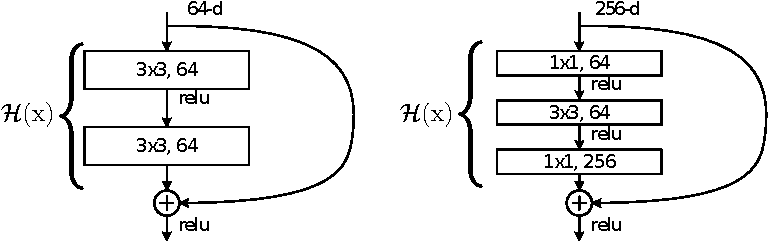
\includegraphics[width=0.85\linewidth]{resnet}
			\caption{ResNet blocks (\citet{resnet})
				\todo{Add \(\mathcal{H}(\ve{x})\) on the schema and small explanation.}
				\label{fig:resnet}
			}
		\end{figure}


	%----------------------------------------------------------------------------------------

	\subsection{Region proposals}\label{sec:frcnn_rpn}


	%----------------------------------------------------------------------------------------

	\subsection{Prediction and classification}\label{sec:frcnn_classif}

%========================================================================================


\section{Training data}\label{sec:detection_data}



%========================================================================================


\section{Connectionist Text Proposal Network}\label{sec:ctpn}


%----------------------------------------------------------------------------------------
